% !TEX root =  ../main.tex
\section{Results}
\label{sec:results}
In this section we present some of the results obtained with our planner. The complete sequences are shown in the companion video.
Specifically, we demonstrate the planner for two really different robots, in a large variety of environments: the humanoid HRP-2 and the quadruped HyQ.
Finally, a last example suggests possible applications to dexterous manipulation.

At the end of the video, we validate our contact plans by exhibiting a solution to the interpolation problem $\mathcal{P}_3$ for these scenarios.

At the end of this section, we discuss the role of the parameters of our framework. We then provide the \textit{interactive} computation times obtained in each case.
We also compare the times obtained with HRP-2 with respect to previous works.

These scenarios complement the ones demonstrated on virtual avatars (Figure~\ref{fig:robots_old}) in our previous ISRR paper~\citep{tonneauisrr15} and video\footnote{\url{http://youtu.be/LmLAHgGQJGA}}.
%~ (Figure~\ref{fig:robots_old}).
 %~ We invite the interested reader to watch the ISRR video (\url{http://youtu.be/LmLAHgGQJGA}), and 
%~ to refer to the previous paper for a discussion on these results.

%~ We say that the planning is \gls{interactive} when the computation time for one step is lesser than the
%~ time to execute it. We arbitrarily approximate this time to one second.

\begin{figure}[t]
\centering
  \begin{overpic}[width=1\linewidth]{figures/robots_old}
		%~ \put (5,) {1)} 
		%~ \put (37,) {2)} 
		%~ \put (68,) {3.a)} 
		%~ \put (5,27) {3.b)} 
		%~ \put (37,27) {4.a)} 
		%~ \put (68,27) {4.b)} 
	\end{overpic}
\caption{Virtual avatars in various scenarios demonstrated in our conference paper.}
		   \label{fig:robots_old}
\end{figure}

\subsection{Description of the scenarios}
In all the scenarios considered, the formulation of the problem is always the same:
a start and goal root configurations are provided as input.
The framework computes the initial contact configuration, and outputs a sequence of contact configurations connecting it to the goal.
In each scenario we detail the contacts involved and the heuristics chosen (either $h_{\textrm{\it EFORT}}$, $h_{vel}$ or $h_{w}$, all of which are defined in the Appendix~\ref{sec:heuristics}).
 %~ and the constraints on the reachable workspaces (for instance in all the scenarios, the reachable workspaces of the legs of HRP-2 are always required to intersect with the environment). 
%~ The companion video presents the complete contact sequence obtained in all these scenarios.

% \subsubsection*{Truck egress (Figure~\ref{res_truck_pres} and Figure~\ref{res_truck_bd}) -- Humanoid and insectoid robots.}
%\subsubsection*{Truck egress -- Humanoid and insectoid robots (Figure~\ref{res_truck_bd}).}
\subsubsection{HRP-2 -- Steep staircase (Figure~\ref{fig:stair_robust}):}

\begin{figure}
  \centering
  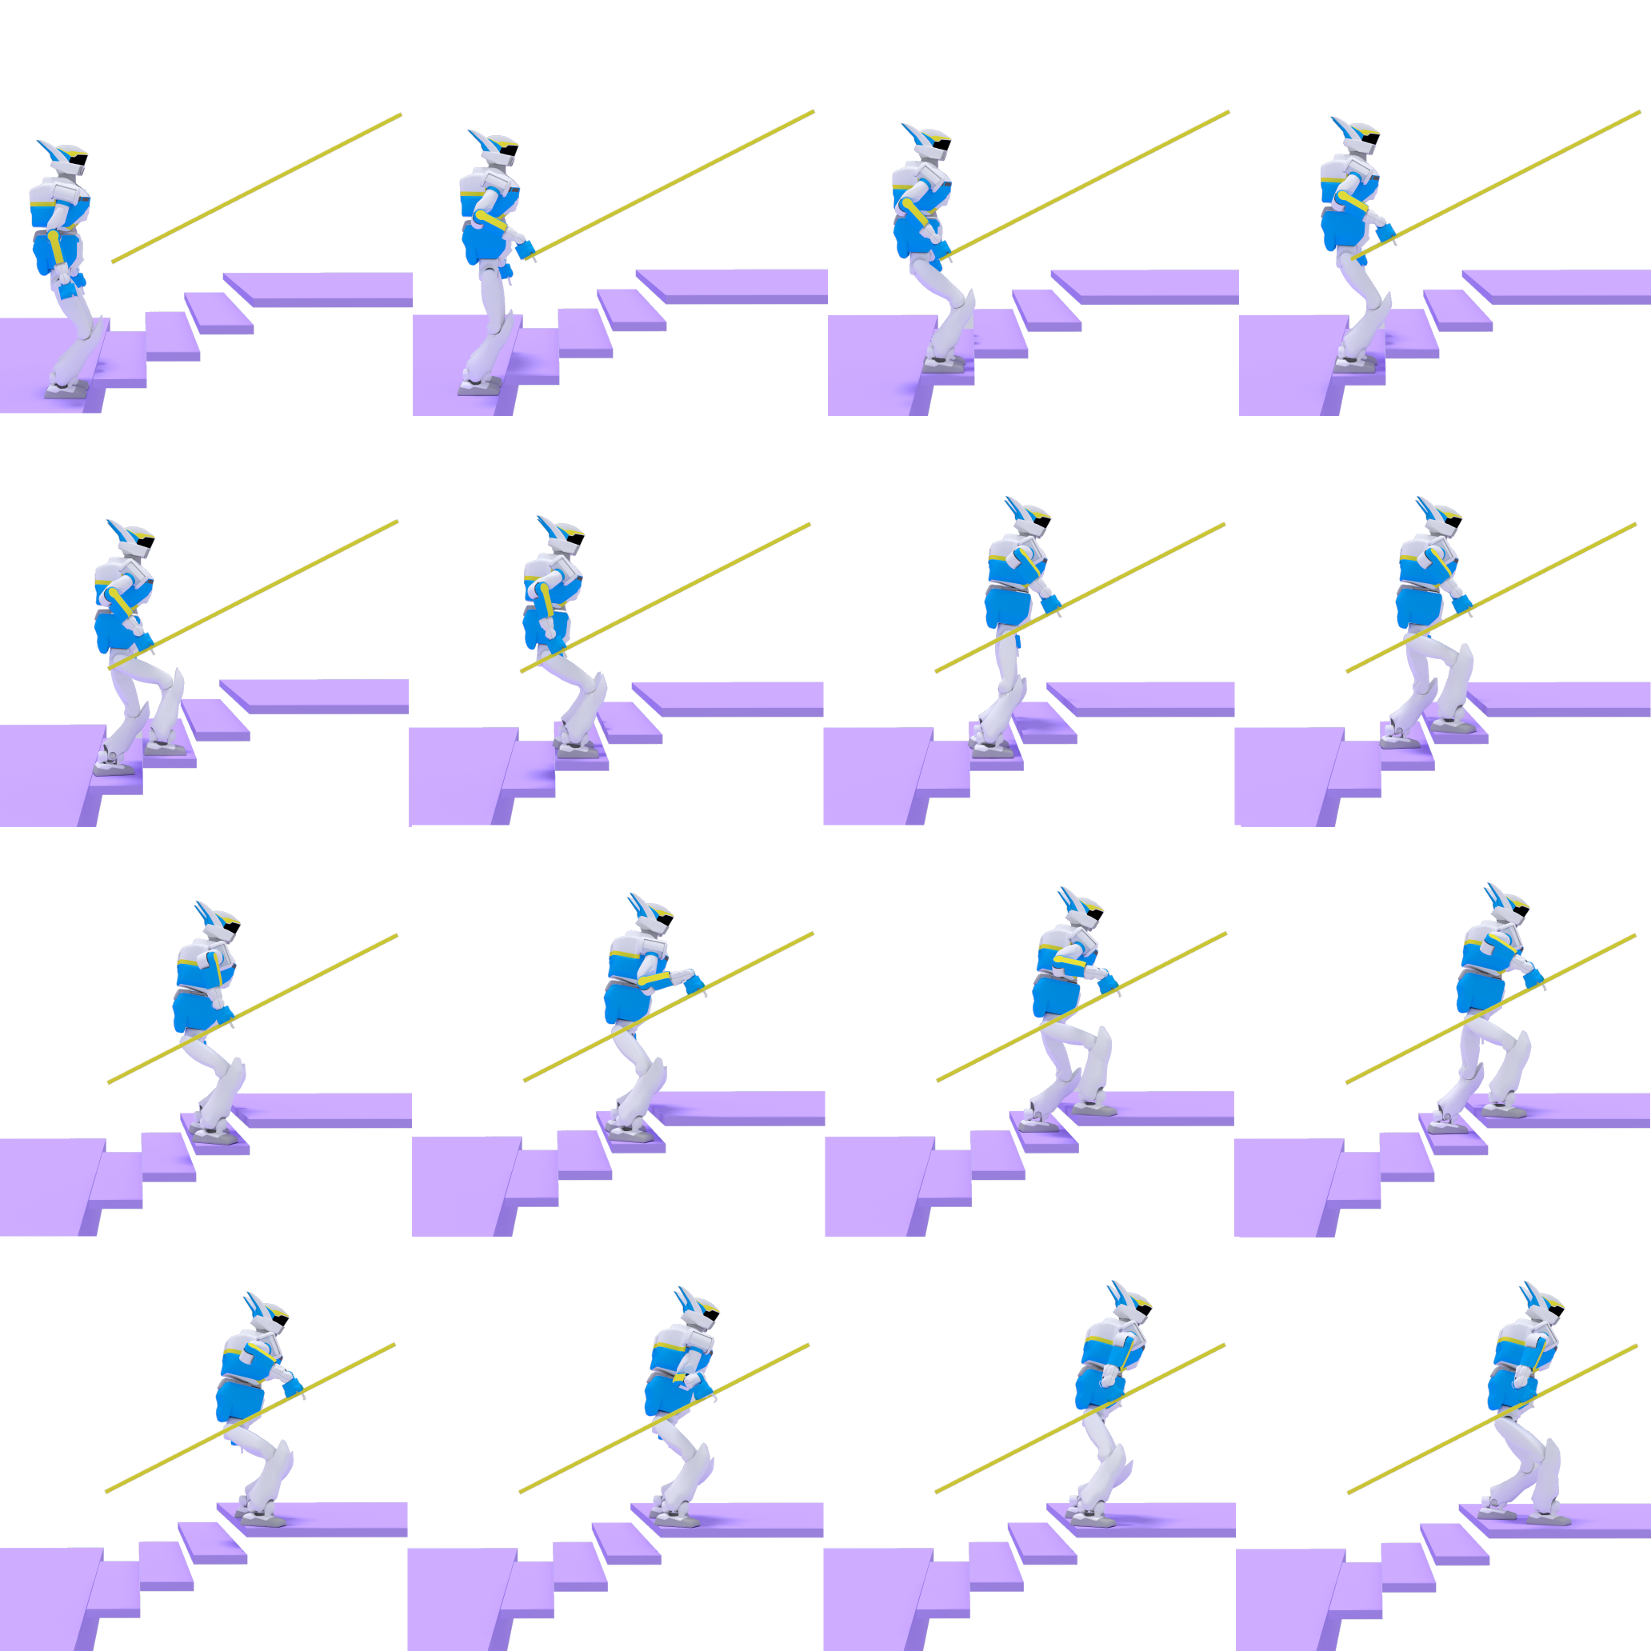
\includegraphics[width=1\linewidth]{figures/stair}
  \caption{
           HRP-2 in the steep stair climbing scenario. }
		   \label{fig:stair_robust}
\end{figure}

The goal is to climb three 15-cm high steps.

\noindent\textbf{Contacts involved:} Feet and right arm.

\noindent\textbf{Heuristics:} The manipulability $h_w$ is chosen for the feet; $h_{\textrm{\it EFORT}}$ is chosen for the right arm.
%~ Regarding equilibrium, the video demonstrates two sequences computed for two different threshold values of $b_0$: $0$ and $2$ (Figure~\ref{fig:stair_robust}). 

%~ \noindent\textbf{Observations:}
%~ This scenario illustrates best the importance of the equilibrium-robustness criterion.
%~ With a robust approach, more states are required to reach the last step (15 rather than 13 in average).
%~ However, when the last step is reached by both feet, in the nonrobust case the contacts are extremely close to 
%~ the cone limits (Figure~\ref{fig:stair_comp}).
%~ 
%~ 
%~ The geometry of the environment is easily addressed by our planner, and the contact planning is several times faster than real time in this scenario.
%~ 
%~ Again, the interpolation motion between the contact steps is out of the scope of this paper. However it should be noted that the computed plan in this scenario has been executed successfully on the robot (\url{http://youtu.be/YjL-DBQgXwk#t=0m28s}).
%~ 
%~ \begin{figure}
  %~ \centering
  %~ \begin{overpic}[width=0.5\linewidth]{figures/stair_robust}
		%~ \put (17,5) {\small{\color{red}$b_0 = 0.23$}} 
		%~ \put (79,5) {\small{\color{green}$b_0 = 6.16$}} 
	%~ \end{overpic}
  %~ \caption{
           %~ Evaluation of the robustness $b_0$ of two contact configurations. Although in equilibrium, the left configuration is on the verge of slipping.}
		   %~ \label{fig:stair_comp}
%~ \end{figure}

\subsubsection{HRP-2 -- Standing up (Figure~\ref{fig:standing}):}
From a bent configuration, the robot has to stand up using a wall as support, and climbing a 25-cm high step.

\begin{figure}
  \centering
  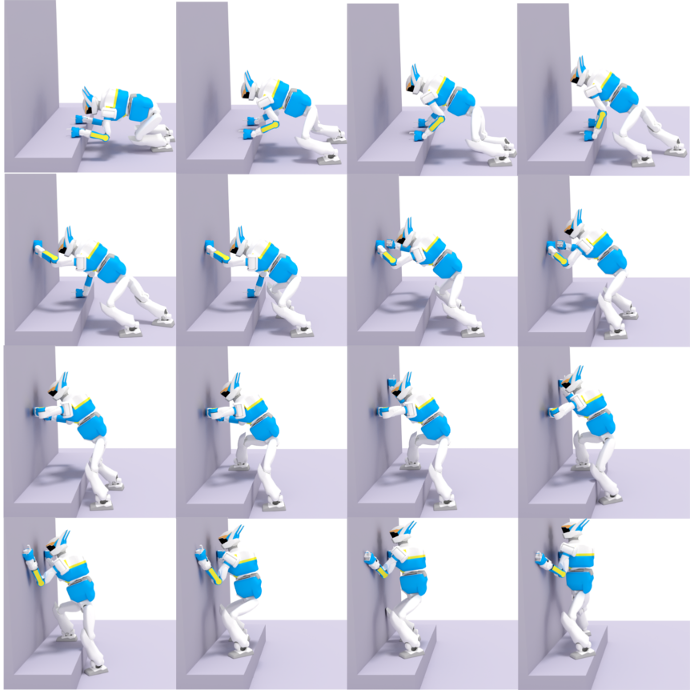
\includegraphics[width=1\linewidth]{figures/standing}
  \caption{
           HRP-2 in the standing scenario. }
		   \label{fig:standing}
\end{figure}


\noindent\textbf{Contacts involved:} All (both feet and hands).

\noindent\textbf{Heuristics:} $h_w$ for the feet, $h_{\textrm{\it EFORT}}$  for the hands.

%~ \noindent\textbf{Observations:} The scenario illustrates well the acyclic aspect of the planning. For instance, in the four first frames of Figure~\ref{fig:standing}, we can see that the right foot
%~ is moved twice, with the left foot in between, before the configuration allows HRP-2 to move its hand.
%~ Because the contacts are tried in a FIFO manner, the fact that the output contact sequence is acyclic shows that a cyclic approach (with a finite state machine for instance) is not sufficient
%~ for the computed path. The reason for this is not reachability, but equilibrium. The planning is slower than for the stair scenario (because the contact generation fails more),
%~ though it remains compatible with \gls{interactive} performances. % \adnote{Maybe define what you mean by 'interactive' and 'real-time' at some point.}


\subsubsection{HRP-2 -- Polaris car egress (Figure~\ref{fig:car}):}
In this scenario inspired from the DRC car egress HRP-2 has to step out of the Polaris car.

\begin{figure}
  \centering
  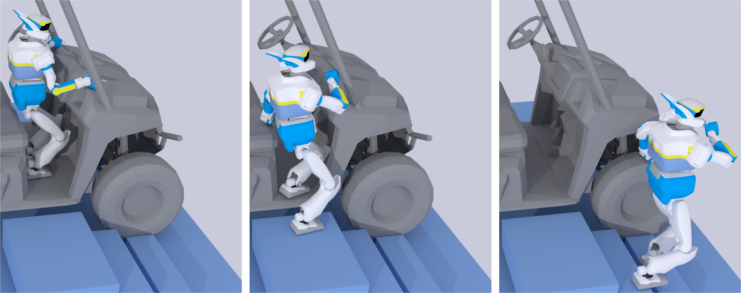
\includegraphics[width=1\linewidth]{figures/polaris}
  \caption{
           Selected frames from the polaris egress scenario. }
		   \label{fig:car}
\end{figure}


\noindent\textbf{Contacts involved:} All (both feet and hands).

\noindent\textbf{Heuristics:} $h_w$.

%~ \noindent\textbf{Observations:} The difficulty of this scenario lies in the strong reduction of the reachable workspace induced 
%~ by the extreme proximity of all obstacles. The planner is able to find a sequence, that consists in many steps.
%~ The proximity of the obstacles invalidate a large number of contact candidates because of collisions. To avoid breaking more than one contact between each step, the motion has to be decomposed into a large number of steps (61 in average).
%~ While this scenario is the slowest to solve, the planner still computes a solution \glslink{interactive}{interactively}.


\subsubsection{HyQ -- DRC-style rubble (Figure~\ref{fig:darpa})}
The quadruped robot must cross a rubble composed of bricks rotated at different angles and directions.

\begin{figure}
  \centering
  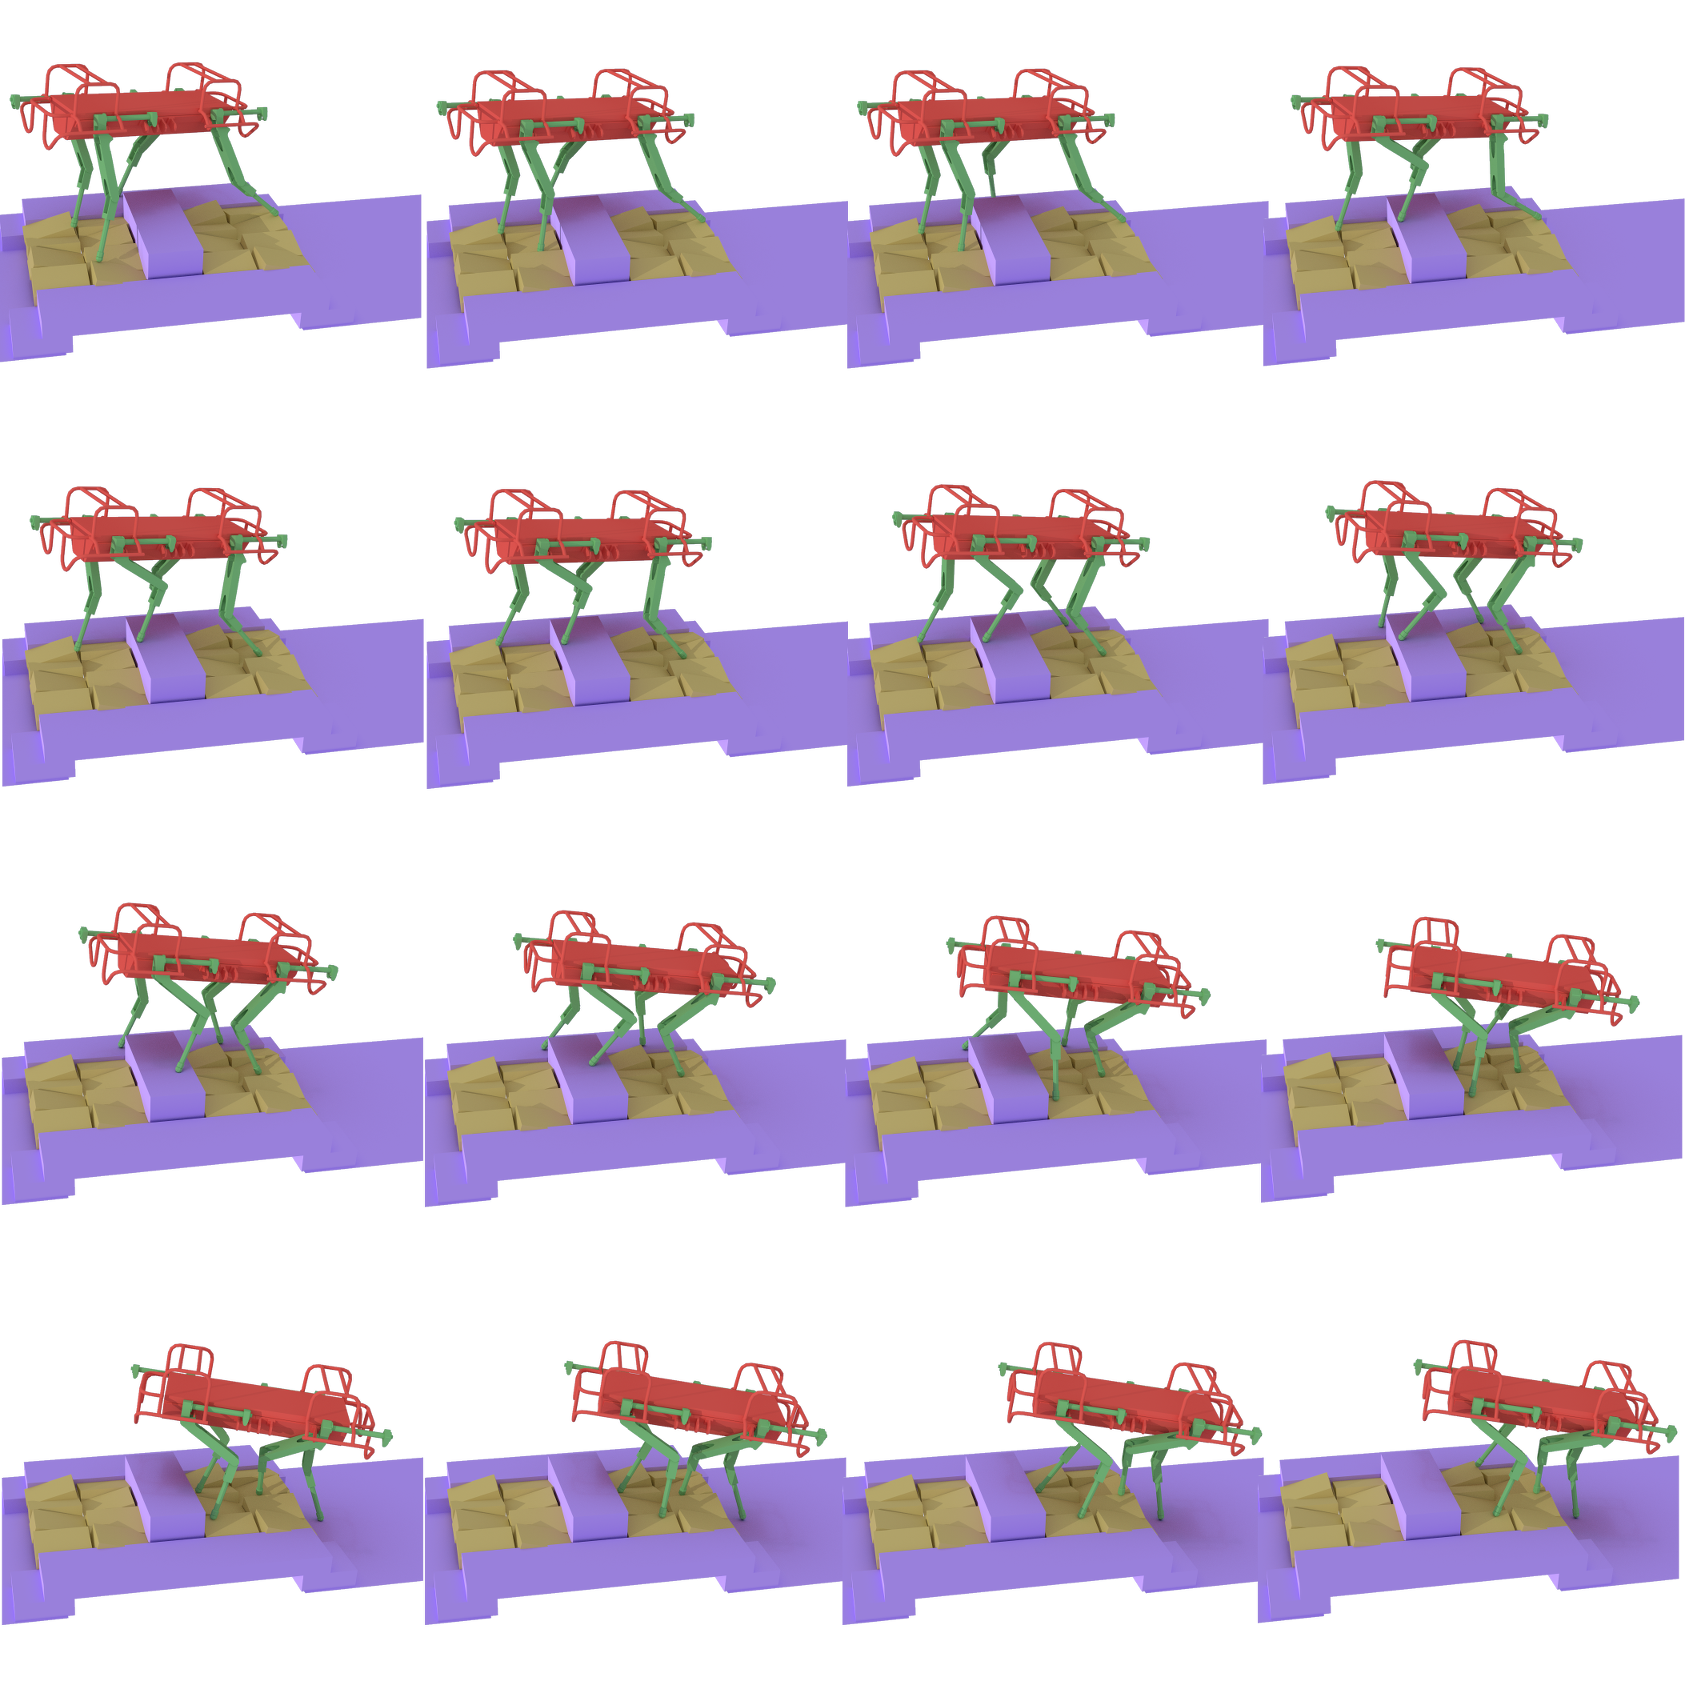
\includegraphics[width=1\linewidth]{figures/darpa}
  \caption{
           Robust crossing of rubbles by HyQ. }
		   \label{fig:darpa}
\end{figure}


\noindent\textbf{Contacts involved:} All (the 4 legs).

\noindent\textbf{Heuristics:} $h_w$ for all legs. The robustness threshold $b_0$ is set to $20$.

%~ \noindent\textbf{Observations:} In this context, setting up a really important minimum value for $b_0$ is possible due to the high
%~ stability of the HyQ robot, and results in more contact switches, in exchange for safety. The guide path-planning in this scenario takes a few seconds in average, more than
%~ in any other scenarios. This is explained by the necessity of discovering a safe way to ``climb down'' the rubble. In this part of the planning, the constraint that the 4 reachable workspaces of all legs must collide with the environment at all times is hard to respect, but enforces the equilibrium of HyQ. %\adnote{Why do not relax this constraint and require only 3 legs?} 
%~ Again, the computation times remain however \gls{interactive}.

\subsubsection{HyQ -- Obstacle race (Figure~\ref{fig:HyQ_bridge} and~\ref{fig:HyQ_obs}):}
In this long scene, HyQ has to cross a 55-cm large hole, followed by a narrow ``bridge'', only 25-cm large.

\begin{figure}
  \centering
  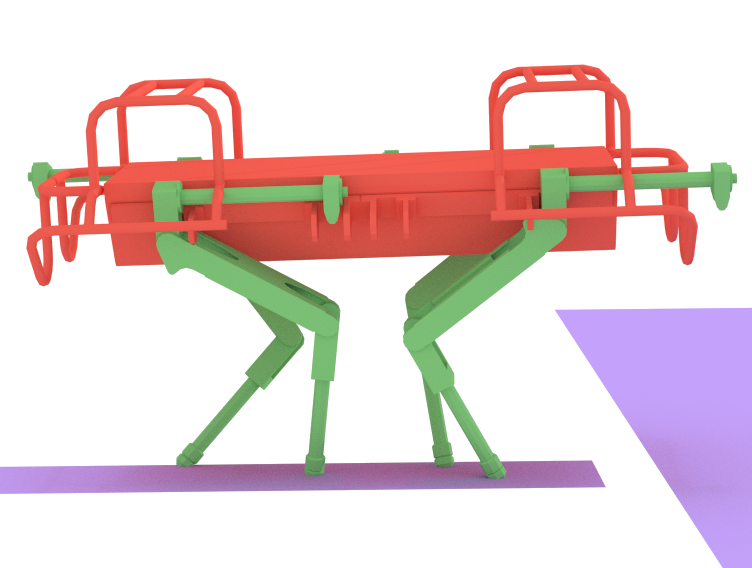
\includegraphics[width=0.4\linewidth]{figures/HyQ_bridge}
  \caption{
           HyQ crossing a narrow bridge. }
		   \label{fig:HyQ_bridge}
\end{figure}

\begin{figure}
  \centering
  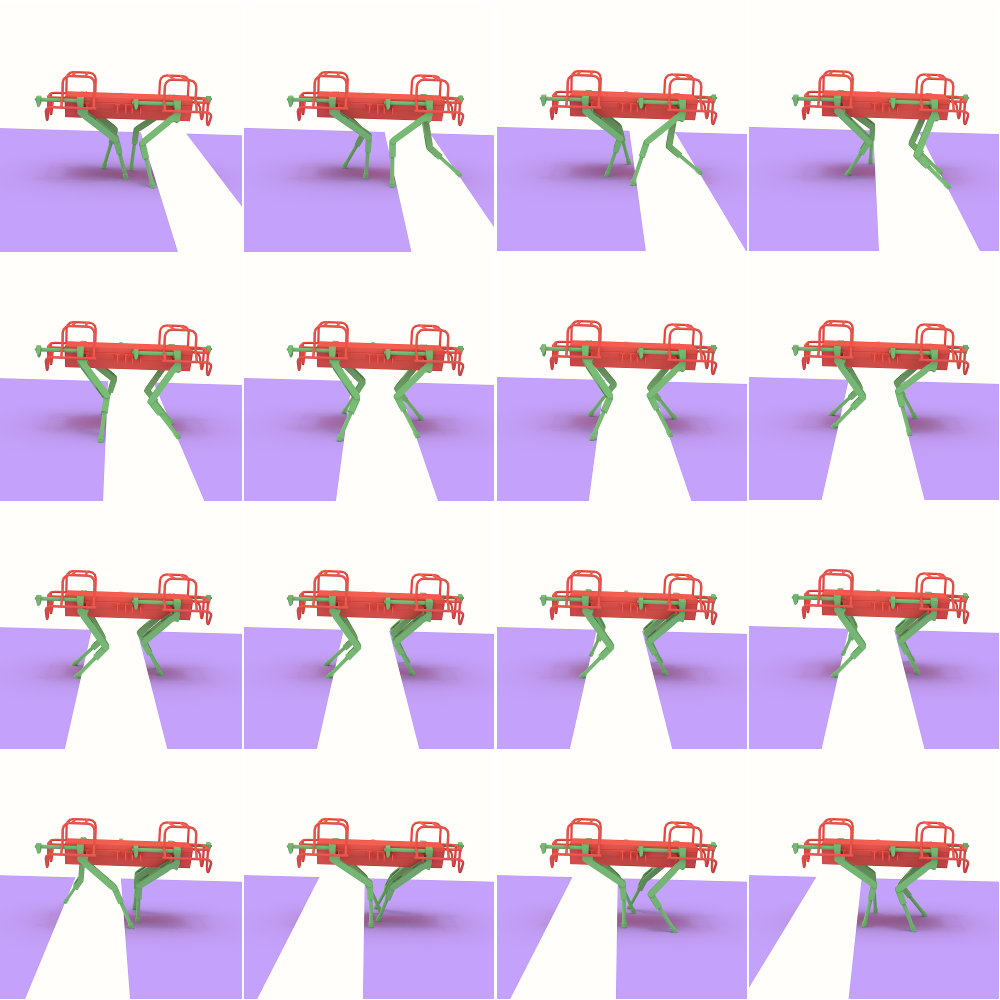
\includegraphics[width=1\linewidth]{figures/HyQ_obs}
  \caption{
           Crossing a hole contact sequence for HyQ. }
		   \label{fig:HyQ_obs}
\end{figure}



\noindent\textbf{Contacts involved:} All (the 4 legs).

\noindent\textbf{Heuristics:} $h_w$ for all legs. The robustness threshold $b_0$ is set to $10$.

%~ \noindent\textbf{Observations:} Despite the apparent simplicity of the scene, this scenario is a hard case for a contact planner.
%~ While finding a guide path above the hole is easy for the guide planner, finding a sequence of contacts that allows for equilibrium is not trivial.
%~ Second, the narrow bridge is hard both for the planner and the contact generator: to make sure that equilibrium is preserved along the traversal,
%~ the bridge must be approached with the appropriate angle.
%~ The difficulty is illustrated in Figure~\ref{fig:HyQ_obs}, where several feet rearrangements are required to cross the hole (although the video shows this best).
%~ The planner however succeeds in finding a feasible sequence in the end, again with \gls{interactive} computation times.

\subsubsection{HRP-2 -- Path re-planning (Figure~\ref{fig:re-planning}):}
In this long scene, HRP-2 plans a path through several obstacles. The scene is edited during the execution of the motion: a stair is added,
some stepping stones are removed, and part of the final staircase is deleted. All these modifications require re-planning.


\begin{figure}
  \centering
  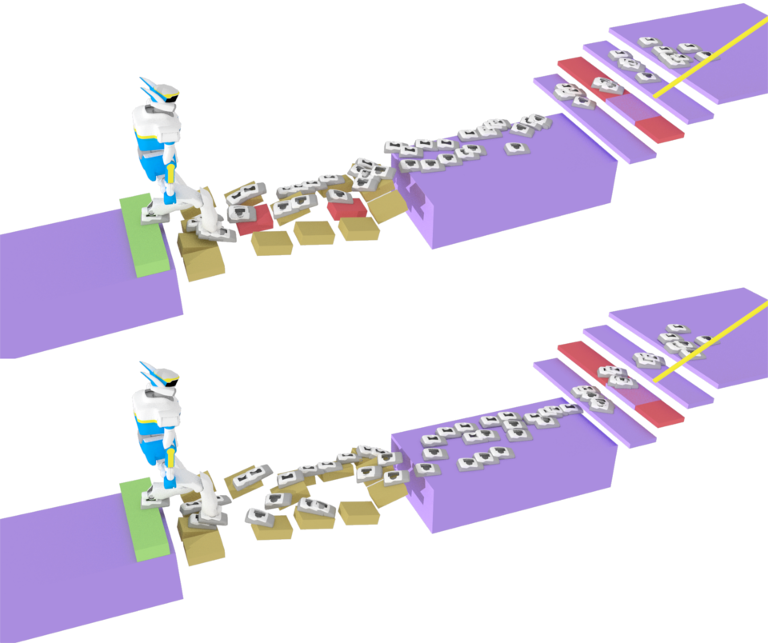
\includegraphics[width=0.7\linewidth]{figures/replanning}
  \caption{
           HRP-2 in the re-planning scenario. After the red step stones are removed, a new sequence of contacts is re-planned. Hand contacts
           are not presented here for readability.}
		   \label{fig:re-planning}
\end{figure}

\noindent\textbf{Contacts involved:} Feet and the right arm.

\noindent\textbf{Heuristics:} $h_w$  for all legs. $h_{\textrm{\it EFORT}}$  for the right arm. The robustness threshold is set to $2$.

%~ \noindent\textbf{Observations:} This scenario is designed to illustrate concretely the computation times of the planner.
%~ In the video, the footsteps indicating the contact sequence appear at the average speed of their computation (including the guide-path planning).


\subsubsection{3-fingered hand -- Manipulation of a pen (Figure~\ref{fig:penrot}):}
This scenario is proposed to illustrate the generality of our approach: we consider a manipulation task for a robotic hand and use
our contact planner to compute a contact sequence for the fingers, considered as effectors (Figure~\ref{fig:penrot}).
Although we do not address the hard issue of accounting for rolling motions, the planner is able to compute the shown sequences in less than 5 seconds.

\begin{figure*}
\centering
  \begin{overpic}[width=1\linewidth]{figures/penrot}
	\end{overpic}
\caption{Contact sequence found for a pen manipulation in a zero gravity environment.}
		   \label{fig:penrot}
\end{figure*}

 
\noindent\textbf{Contacts involved:} Three finger-tips.

\noindent\textbf{Heuristics:} $h_{\textrm{\it EFORT}}$ for all fingers.
 
 
\subsection{Role of the main parameters} \label{sec:influence}
We discuss the factors that influence the outcome of our planner: the root scaling factor $s$ (Section~\ref{sec:scaling}), the heuristics for
contact generation (Appendix~\ref{sec:heuristics}), and lastly, the discretization step for the guide path. The appropriate value for these parameters
is computed empirically based on use-case analysis or trials and errors.
 
\subsubsection{Choosing the scaling factor $s$:} \label{sec:params}
%~ \deladp{To find a convenient value $s^*$ of $s$, we proceeded as follows. }
For several values of $s$, we generated $10 000$ configurations. 
We then computed the sensitivity of the reachability condition (percentage of configurations in $C_{Reach}^0$, effectively belonging to \gls{$C_{Contact}^0$}).
Similarly we computed the specificity of the condition (percentage of configurations \textbf{not} in $C_{Reach}^0$, effectively \textbf{not} belonging to \gls{$C_{Contact}^0$}).
The obtained results for HRP-2 are shown in Table~\ref{tab:scale}, averaged over all scenes (except for the car egress: in this scenario, 
statistical tests are not really conclusive since we are only interested in a small area of the environment).

As it can be expected, the scaling results in a high increasepercentage of the sensitivity, with a decrease of the specificity.
For HRP-2 we decided to set $s^*=1.2$.
%~ , and was also effective for the car egress scenario. 

\begin{table}
\centering
\footnotesize
\begin{tabular}{c | c | c}
   Value of $s$ &  Sensitivity & Specificity\\
 \hline
   1   & 76\% & 100 \%\\
   1.1& 88\% & 96\% \\
   1.15& 93\% & 94\%\\
   1.2 & 97\% & 92.5\%\\
   1.25& 98\% & 91.7\%\\
   1.5 & 99\% & 90.5\%\\
 \end{tabular}
\caption{Sensitivity and specificity values of the reachability condition, depending on the scaling value $s$ of $W^0$.}
\label{tab:scale}
\quad
\end{table}

\subsubsection{Choosing the heuristics:} \label{sec:heuristichoices}
In our conference paper~\citep{tonneauisrr15}, the computed motions were generated using the EFORT heuristic.
EFORT is designed for tasks requiring to exert important forces (such as pushing / pulling / climbing). 
In locomotion tasks, such as the stair scenario, one issue with EFORT is that it tends to generate
configurations close to singularities (and joint limits). While this does not significantly impact
the generation of the plan, the resulting interpolation turned out to be harder.
For this reason, we prefer to use our manipulability-based heuristic for the legs of the robot, but we still
use EFORT for the arms, which results in less contact repositionings.

%~ \subsubsection{On the robustness equilibrium criterion:} \label{sec:parrob}
%~ Robustness is really important when considering practical applications on the robot, to account 
%~ for the various uncertainties that result from environment and state estimation. However,
%~ maximizing the robustness criterion is often not optimal, because the resulting configurations may be too conservative, thus not favoring the motion. In our experiments, we choose not to maximize the robustness,
%~ but to empirically set a robustness threshold value under which a configuration is not considered to be in
%~ static equilibrium (If no candidate reaches the threshold, instead of failing, the algorithm can eventually return the ``more robust'' configuration
%~ found). Currently for HRP-2, a threshold value of 2 subjectively gives the best results in the considered scenarios, while 10 seems to be a good choice for HyQ. Both values do not
%~ significantly slow down the planning times.

\subsubsection{Discretization of the guide path:} \label{sec:disc}
The discretization step is a user-defined, fixed parameter. The step
has an influence on the output of the planner: if too large steps are taken,
the planner may fail since we impose the constraint that only one contact change might occur
between two consecutive steps. On the other hand, a small step will not impact the success rate of the planner, 
but may generate unnecessary states. In most scenarios the torso of HRP-2 moves about 15 cm between two postures, but only 3 cm
for the car egress scenario to handle the geometry of the polaris.
For future work, we would like to automatically adapt the size of the discretization step to the complexity of the environment.

\subsection{Performance analysis} \label{sec:perf}
To analyze performance, we ran the planner 1000 times for each considered scenario.
We measured the computation time spent in each part of the algorithm, and analyzed their success rate.


\begin{table*}
\centering
\footnotesize
\begin{tabular}{ >{\centering\arraybackslash}m{37pt} | >{\centering\arraybackslash}m{57pt} | >{\centering\arraybackslash}m{65pt} | >{\centering\arraybackslash}m{70pt} | >{\centering\arraybackslash}m{73pt} | >{\centering\arraybackslash}m{80pt} | >{\centering\arraybackslash}m{10pt}}
  Scenario (nb steps) &  Complete guide generation (ms) & Static equilibrium (ms) & Collision (ms) & Inverse Kinematics (ms) & Total generation time (ms) & Time per step (ms)\\
 \hline
   Stairs (18) 	& 5 -- \textbf{6} --  18 		 & 13 --  \textbf{32} -- 329   	& 1 --  \textbf{4} -- 38 & 26 --  \textbf{127} -- 1345 & 92 --  \textbf{261} -- 2174 & \textbf{15} \\
   Standing (24)& 65 -- \textbf{1086} --  5227   & 27 --  \textbf{144} -- 338   & 2 --  \textbf{12} -- 37 & 144 --  \textbf{1046} -- 2374 & 371 --  \textbf{2257} -- 7671 & \textbf{94}  \\
   Car (86)& 320 -- \textbf{6971} --  44002 & 409 --  \textbf{1766} -- 14752   	& 297 -- \textbf{1187} -- 8483 & 3154 --  \textbf{15323} -- 165541 & 5834 --  \textbf{31391} -- 281000 & \textbf{365}\\
   Rubble (82)& 37 -- \textbf{573} --  1685 & 583 --  \textbf{2714} -- 9459 & 491 --  \textbf{1971} -- 6273 & 269 --  \textbf{706} -- 3118 & 1811 --  \textbf{7195} -- 23241 & \textbf{86} \\
   Race (134)& 14 -- \textbf{51} --  125 & 455 --  \textbf{1359} -- 21045   & 397 --  \textbf{923} -- 9924 & 228 --  \textbf{471} -- 5415 & 1436 --  \textbf{3343} -- 41446 & \textbf{25}
 \end{tabular}
\caption{minimum, \textbf{average} and worst time (in ms) spent in the generation process for each scenario and each critical part of the generation process (not all parts are timed,
thus the average total computation time is higher than the sum of each part). The last
column indicates the average time necessary to compute one contact transition. }
\label{tab:requestime}
\quad
\end{table*}


\begin{table}
\centering
\begin{tabular}{ l | c}
  &  Path planning success rate \\
 \hline
   Stairs     	& 100\% \\
   Standing			& 68\% 	\\
   Car 			& 77\% 	\\
   Rubble 				& 97\% 	\\
   Race        & 88.0\% 	\\
 \end{tabular}
\caption{ Percentage of successful complete contact planning rates for each scenario, rounded to the first decimal.}
\label{tab:sucess_planning}
\quad
\end{table}

\begin{table}
\centering
\begin{tabular}{ l | >{\centering\arraybackslash}m{65pt} | >{\centering\arraybackslash}m{35pt} | >{\centering\arraybackslash}m{35pt} | c}
  &  Equilibrium success rate & Kinematic failure & Equilibrium failure \\
 \hline
   Steep stairs 	& 99.5\%  & 0.1\% 	& 0.4\% \\
   Standing up 		& 87.8\%  & 6.1\% 	& 6.1\% \\
   Car egress 		& 66.2\%  & 15.9\% 	& 17.9\% \\
   Rubble 			& 97.54\% & 0.16\% 	& 2.3\% \\
   Obstacle race 	& 92.4\%  & 0.15\% 	& 7.45\% \\
 \end{tabular}
\caption{Success rates obtained for the generation of static equilibrium contact configurations for each scenario, rounded to the first decimal. Column 1 indicates 
indicates the rate of contact generation that suceeeded. In the cases where the generation fails, it can be
either a kinematic issue (column 2), or because no contact configuration led to a static equilibrium configuration (column 3). Note that a failure in the contact generation
is not equivalent to a failure of the contact planning algorithm.}
\label{tab:requestpercent}
\quad
\end{table}

\subsubsection{Computation times:}
Table~\ref{tab:requestime} summarizes the computation times.

For HRP-2, most of the time was spent performing inverse kinematics.
This is not surprising considering the number of calls to the methods: IK projection is used intensively to maintain contact continuity between two postures; 
it is also applied every time a new candidate needs to be evaluated. In particular for the car egress scenario,
the kinematic constraints are very demanding to avoid collisions.

On the other hand for HyQ most of the time is spent testing the static equilibrium of the candidate configurations.

In all scenarios, one can observe that the average computation time for one single step is largely below one second,
thus allowing to consider \gls{interactive} applications and online autonomous planning of the robot motion.


\subsubsection{Success rates:}
Table~\ref{tab:sucess_planning} summarizes the successful planning rates.
Despite the complexity of the scenarios addressed, as well as the approximations made in our formulation, our planner succeeded in the large majority of cases.

Table~\ref{tab:requestpercent} presents the rate of successful contact generation. Note that a failure in contact generation for a root configuration is not equivalent to a failure in the contact plan. It simply means that another limb was tested for contact generation for the same root configuration.
As expected, the more constrained scenario, the car egress, provides the less satisfying results, despite the high success rate of the planner.

These results confirm that our approach provides a satisfying compromise between completeness and efficiency, thus allowing to consider online planning
while controlling the robot. Indeed, when the contact planning fails, it fails rapidly. This allows us to rapidly re-plan with a reasonable chance of success.
The most efficient (and immediate) approach to obtain a valid contact plan as fast as possible would be to launch in parallel several instances of the planner (our current implementation is single-threaded) and to use any successful result as a plan for solver $\mathcal{P}_3$.


\begin{table}
\centering
\begin{tabular}{ c | c | c }
 Scenario & Method  & Computation time \\
 \hline
   \multirow{3}{*}{Stair 20 cm} & Hauser~\cite{Hauser06usingmotion} &  5.42 min  \\							 
							  & Mordatch et al.\cite{Mordatch:2012:DCB:2185520.2185539} & 2 to 10 min \\
							 & \textbf{Ours} + \cite{Carpentier2016}  & \textbf{$ <$ 2s} \\
 \hline
   \multirow{3}{*}{Stair 30 cm} & Hauser~\cite{Hauser06usingmotion} &  4.08 min  \\
							 & Mordatch et al.\cite{Mordatch:2012:DCB:2185520.2185539} & 2 to 10 min \\
							 & \textbf{Ours}  & \textbf{$ <$ 2s}   \\
 \hline
   \multirow{3}{*}{Stair 40 cm} & Hauser \cite{Hauser06usingmotion} &  10.08 min  \\
							 & Mordatch et al.\cite{Mordatch:2012:DCB:2185520.2185539} & 2 to 10 min \\
							 & \textbf{Ours}   & \textbf{$ <$ 5s}   \\
 \hline
   \multirow{2}{*}{Table (car) egress} & Bouyarmane et al.~\cite{Bouyarmane2009, DBLP:conf/iser/EscandeKMG08} & 3.5 hours  \\
							 & \textbf{Ours}  & \textbf{$<$ 60 s} \\
							 
 \end{tabular}
\caption{Comparison between the computation times obtained by our method and previous ones for addressing the whole problem.}
\label{tab:compprev}
\quad
\end{table}

\subsection{Validation of the contact plans, and comparison with previous work} \label{sec:compa}
To validate our plans, we either use the framework proposed in \cite{Carpentier2016} or our own implementation of a $\mathcal{P}_3$ solver, detailed in Appendix~\ref{app:optim}.
The companion video shows the obtained motions.

Few contributions provided computation times on the complete problem. %, necessary to provide comparison between our approaches. 
Furthermore, $\mathcal{P}_3$ remains an open problem in the presence of obstacles. The only valid scenarios addressed completely in previous works are thus the stair-climbing scenarios of different heights proposed by Hauser in \cite{Hauser06usingmotion}, and the table-egress scenario by Escande et al. in~\cite{DBLP:conf/iser/EscandeKMG08}, which we consider to be of similar complexity with respect to the car-egress scenario (we did not consider the stairs in the scene). Both scenarios are tested with HRP-2.

Table~\ref{tab:compprev} presents the computation times for these scenarios, clearly demonstrating that our approach is order of magnitude faster than previous works.



